\hypersetup{
    colorlinks=true,
    linkcolor=blue
}

\chapter{Introduction} \label{ch:introduction}
\begin{center}
  "We really designed the Model S to be a very sophisticated computer on wheels. We view this the same as updating your phone or your laptop. Tesla is a software company as much as it is a hardware company. A huge part of what Tesla is, is a Silicon Valley software company."
  - Elon Musk \cite{ElonMusk}
\end{center}
With these words, Elon Musk, the visionary entrepreneur behind many of the most innovative companies in today's business landscape and co-founder of one of, if not the, most progressive automotive companies of today, namely Tesla, highlighted how the automotive industry is changing dramatically over time, transforming today cars and vehicles from objects in which the fundamental part consists of mechanics components, to ones in which the main focus lies in the simplicity of hardware and the innovation of software.

This shift in paradigm, which is now a reality in the automotive industry, requires significant effort, especially from a security perspective. While a cyber vulnerability in a traditional device like a laptop or smartphone may result in data loss, vulnerabilities in a vehicle's computer system, where software is a fundamental element, can have tragic and even life-threatening consequences. For this reason, addressing security from the design stage is one of the primary objective of this paper.

In order to address and understand the Software Defined Vehicle, which is the most recent expression of software integration in the automobile, it is necessary to delve into the automotive industry and the dynamics that exist with respect to software production. For this reason, in this introduction an overview of the automotive context in which the project is located will be discussed and then the role of the project partner company, which is also a leader in software consulting and development and a partner of major automotive companies, will be detailed. Finally, in conclusion of this chapter, the thesis's key objectives and the practical project that will support this work during the description are shown also giving an introductory overview of the entire work proposed in this thesis project.

\section{Automotive Context}
The automotive industry has stood out for decades as a continuously growing sector, playing a significant role both as an employer for millions of people and as an investor in the research and development of cutting-edge technologies in many fields, including mechanics, materials, and software. Thanks to the presence of the largest automotive companies across Europe, there is a great deal of knowledge in this sector, which represents one of the most crucial areas for the European Union's economy. As can be seen from the table below \ref{tab:VehicleProduction}, the production of total vehicles worldwide has been continuously growing, with the exception of two periods: following the financial crisis of 2007-2008 and following the pandemic of 2020, both events having a very strong impact on the entire global economy and which have had effects on many sectors. In any case, it can be noted that automotive production has resumed strong growth in the last two years.

\begin{table}[htbp]
  \centering
  \caption{World automobile production in million vehicles \cite{automotiveInCentralEurope}}
  \label{tab:VehicleProduction}
  \begin{tabular}{cccc}
    \toprule
    Year & Production (millions) & Change \\
    \midrule
    2007 & 73 266 061 & + 05.80 \% \\
    2008 & 70 520 493 & - 03.70 \% \\
    2009 & 61 791 868 & - 12.40 \% \\
    2010 & 77 857 705 & + 26.00 \% \\
    2011 & 79 989 155 & + 03.10 \% \\
    2012 & 84 141 209 & + 05.30 \% \\
    2013 & 87 300 115 & + 03.70 \% \\
    2014 & 89 747 430 & + 02.60 \% \\
    2015 & 90 086 346 & + 00.40 \% \\
    2016 & 94 976 569 & + 04.50 \% \\
    2017 & 97 302 534 & + 02.36 \% \\
    2018 & 95 634 593 & - 01.71 \% \\
    2019 & 91 786 861 & - 05.20 \% \\
    2020 & 77 621 582 & - 16.00 \% \\
    2021 & 80 145 988 & + 03.25 \% \\
    2022 & 85 016 728 & + 06.08 \% \\
    2023 & 93 546 599 & + 10,03 \% \\
  \bottomrule
  \end{tabular}
\end{table}

In the ever-expanding landscape of the automotive industry, a new frontier has been added in recent years, that of software development, which first arrived in the luxury car markets as optional and marginally relevant systems in the vehicle, and then spread to all types of vehicles, so that today the current challenges for automotive companies extend far beyond the traditional areas of mechanical or material engineering to reach a total and fundamental involvement in the study and innovation of software and hardware components for vehicle construction. 

A look at the intricate network of different components in today's cars, as shown in Figure \ref{fig:VheicleProcessors}, reveals that a vehicle is actually composed of a mosaic of dozens of different systems, which in turn are composed of dozens of processors that interact with each other at different levels, earning today's vehicles the moniker \textit{'Computers on Wheels'}.
\begin{figure}[h]  % 'h' significa che la figura viene posizionata qui
  \centering
  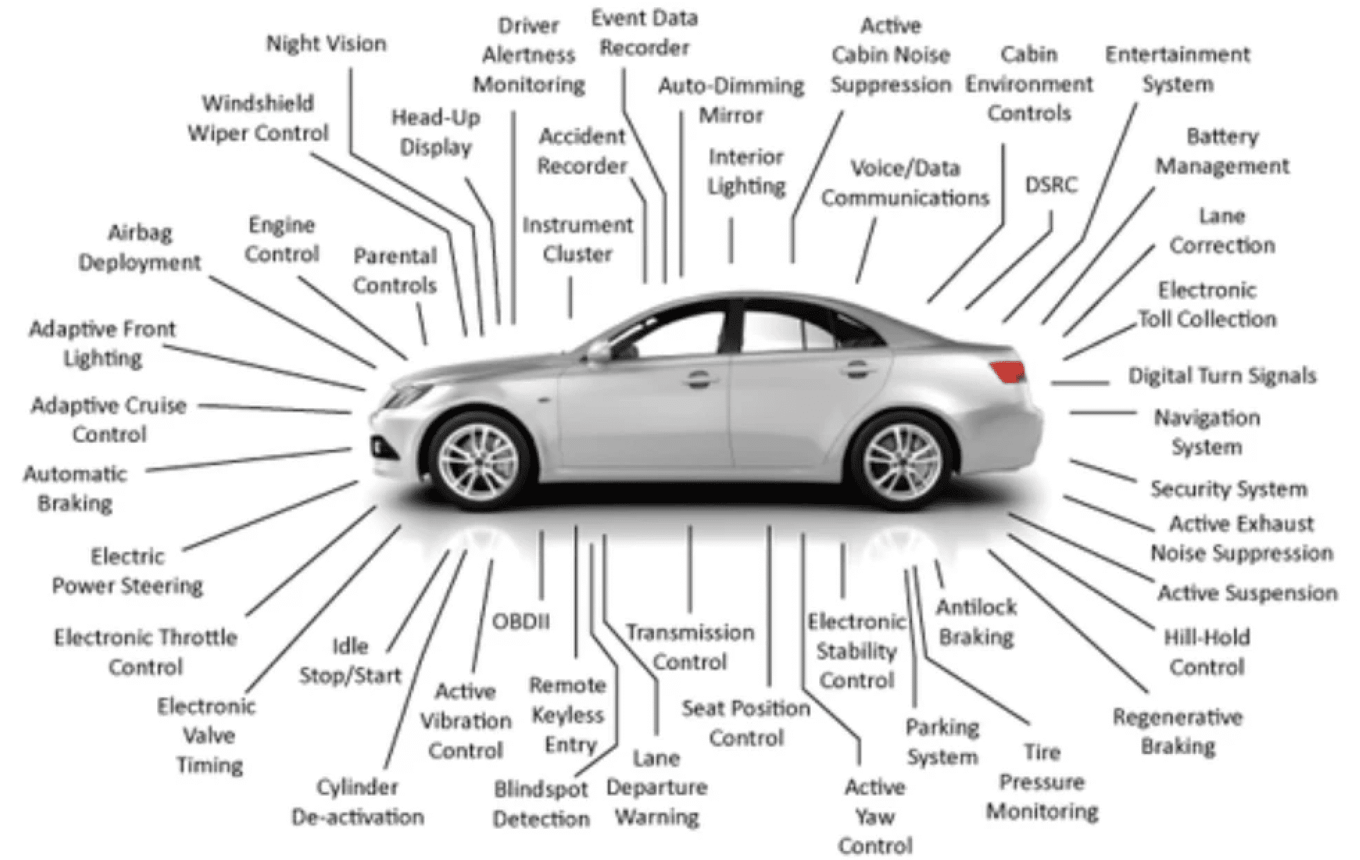
\includegraphics[width=0.9\textwidth]{images/vehicle_processors.png}  % Sostituisci 'nome_immagine' con il nome del tuo file immagine e l'estensione
  \caption{An incomplete overview of computers in a modern car \cite{ieeeSoftwareDefinedVehicle}}
  \label{fig:VheicleProcessors}
\end{figure}

This paradigm shift has been driven in part by the introduction of autonomous driving. To ensure maximum safety, a car must be equipped with dozens of sensors that can constantly collect data about what is happening to the vehicle and its surroundings. The number of these telemetry devices, which are nothing more than specialized IoT devices for the automotive world, also known as Telematic Control Unit (TCU), is expected to grow as autonomous driving technologies advance. In addition to data collection, another key issue is data analysis. Modern vehicles are caught between low-power systems for maximum vehicle efficiency and high-performance systems for analyzing the collected data and making excellent decisions in a short time.

However, the proliferation of processors within vehicles, orchestrating communication to manage diverse components, presents a formidable challenge; each component often integrates a processor with unique logics, diverging from the logics embedded in processors of other components. Complicating matters further, these components are frequently supplied by companies with proprietary management logics, not readily accessible to the automotive companies themselves.

In addressing this intricate scenario, the transformative concept of a Software Defined Vehicle (SDV) comes to the forefront. Defined as "any vehicle that manages its operations, adds functionality, and enables new features primarily or entirely through software"  \cite{blackberrySDV}, the notion of SDV, with all the associated technologies, offers a comprehensive solution to the challenges posed by the intricate interplay of software and hardware in modern vehicles.

One of the main benefits of this innovation in the automotive industry is the ability to have easily manageable systems. In the past, due to their high level of specialization for performance and low power consumption, automotive computer systems were developed and tested directly on the devices themselves, often in a manual way. This resulted in a large consumption of resources and a waste of time. Today, the goal is to have cloud infrastructures that ensure a more agile development and testing process due to the presence of general-purpose systems in the vehicle.

Consequently, the use of Software Defined Vehicle aims to completely separate software and hardware, allowing the production of high-level software on entirely generalized hardware systems. This results in significant savings in terms of time and money for hardware production, along with providing an advantage in terms of security due to the simplification of software.

Another very important aspect of SDV, which will be analyzed in the following chapters, is that since a Software Defined Vehicle is by definition characterized by the ability to dynamically and flexibly update software, this solution offers significant security advantages in several aspects:
\begin{enumerate}
  \item \textbf{Human Safety Critical Security:} From the moment that a vehicle can be classified as safety critical (as it is reported in the standard ISO 26262-1:2018 of the ISO society where is said that "safety is one of the key issues in the development of road vehicles" \cite{ISO26262}), the elimination of software vulnerabilities related to the vehicle's systems is crucial for the overall safety of the vehicle itself.  
  \item \textbf{Intrinsic Software Security:} This approach allows for the prevention and resolution of vulnerabilities unknown at the time of software design, contributing to ensuring a high standard of security. For example, as demonstrated by NIST in the research on the Analysis Of The Impact Of Software Complexity \cite{NISTCodeComplexity}, the increase in software complexity in different cases results in less analyzable programs. In some instances, the same vulnerability analysis tool may detect vulnerabilities, while in others, analyzing the same code, it may not. 
\end{enumerate}

Effectively navigating the development of SDV technology necessitates a collaborative approach across diverse companies, particularly in the realms of hardware and cloud computing. For this reason, many software, hardware, and automotive companies are involved in the development of this innovation, which aims to become a standard in vehicle production for the entire automotive industry.

In order to carry out the research and analysis of the new technologies described above, as well as to get involved in the practical side of things, it was essential to find a company that had both the IT skills needed to interface with cloud technologies and experience in the world of automotive manufacturing and software production. The partner company with which the practical design and implementation of the working explanatory example was carried out is introduced below.
\section{Partner Company}

Leveraging extensive experience in the cloud industry and fostering deep-rooted relationships within the automotive sector, Storm Reply stands out as the ideal choice to lead the project discussed in this thesis. A key player in the Reply group, Storm Reply specializes in designing and implementing innovative Cloud-based solutions and services \cite{StormReplySite}. 

With a broad client base spanning multiple sectors, particularly the automotive industry, the company's expertise played a pivotal role in fully understanding the project's context and internal dynamics. This extensive knowledge provided the cornerstone for the development of a tangible example of the infrastructure.

\begin{figure}[h]  % 'h' significa che la figura viene posizionata qui
  \centering
  
\includegraphics[width=0.3\textwidth]{images/Storm_Reply_logo.png}  % Sostituisci 'nome_immagine' con il nome del tuo file immagine e l'estensione
  \caption{Logo of the partenr company of the project}
  \label{fig:StormReplyLogo}
\end{figure}

Among the main customers in the automotive world of the consulting company, we can mention Ferrari, one of the most important companies in motor sports competitions and in the production of luxury cars, and Stellantis, one of the biggest giants in the automotive industry as well as in the global market. Although different, these two companies interact with Storm Reply to take advantage of its great knowledge in the cloud world and in the management of AWS services. Thanks to the connection with these important companies it was possible to receive essential information for the thesis work.

One great advantage of collaborating with this company is the wide availability of resources, both material and, above all, in terms of experience. As a large IT consultancy company, Reply is divided into many sub-business units, that makes possible the nteraction with various realities, ranging from embedded to low-level development, network and security infrastructure management, and web services management. Furthermore, there is a research and development section called Area 42 where entities can interact and influence each other to create innovative projects.

A point of pride for Storm Reply is its recognition as an Amazon Web Services (AWS) Premier Consulting Partner since 2014, ranking among the top Amazon Partners globally. This distinctive characteristic underscores the decision to develop the infrastructure using Amazon Web Services.

According to the official AWS description page \cite{AWSGlobalInfrastructure} the AWS Cloud spans 102 Availability Zones within 32 geographic Regions around the world and servs 245 countries and territories. With millions of active customers and tens of thousands of partners globally, AWS has the largest and most dynamic ecosystem. AWS is evaluated as a Leader in the 2022 Gartner Magic Quadrant for Cloud Infrastructure and Platform Services (a series of market research reports published by IT consulting firm Gartner that rely on proprietary qualitative data analysis methods to demonstrate market trends, such as direction, maturity and participants), placed highest in Ability to Execute axis of measurement among the top 8 vendors named in the report.

\begin{figure}[h]  % 'h' significa che la figura viene posizionata qui
  \centering
  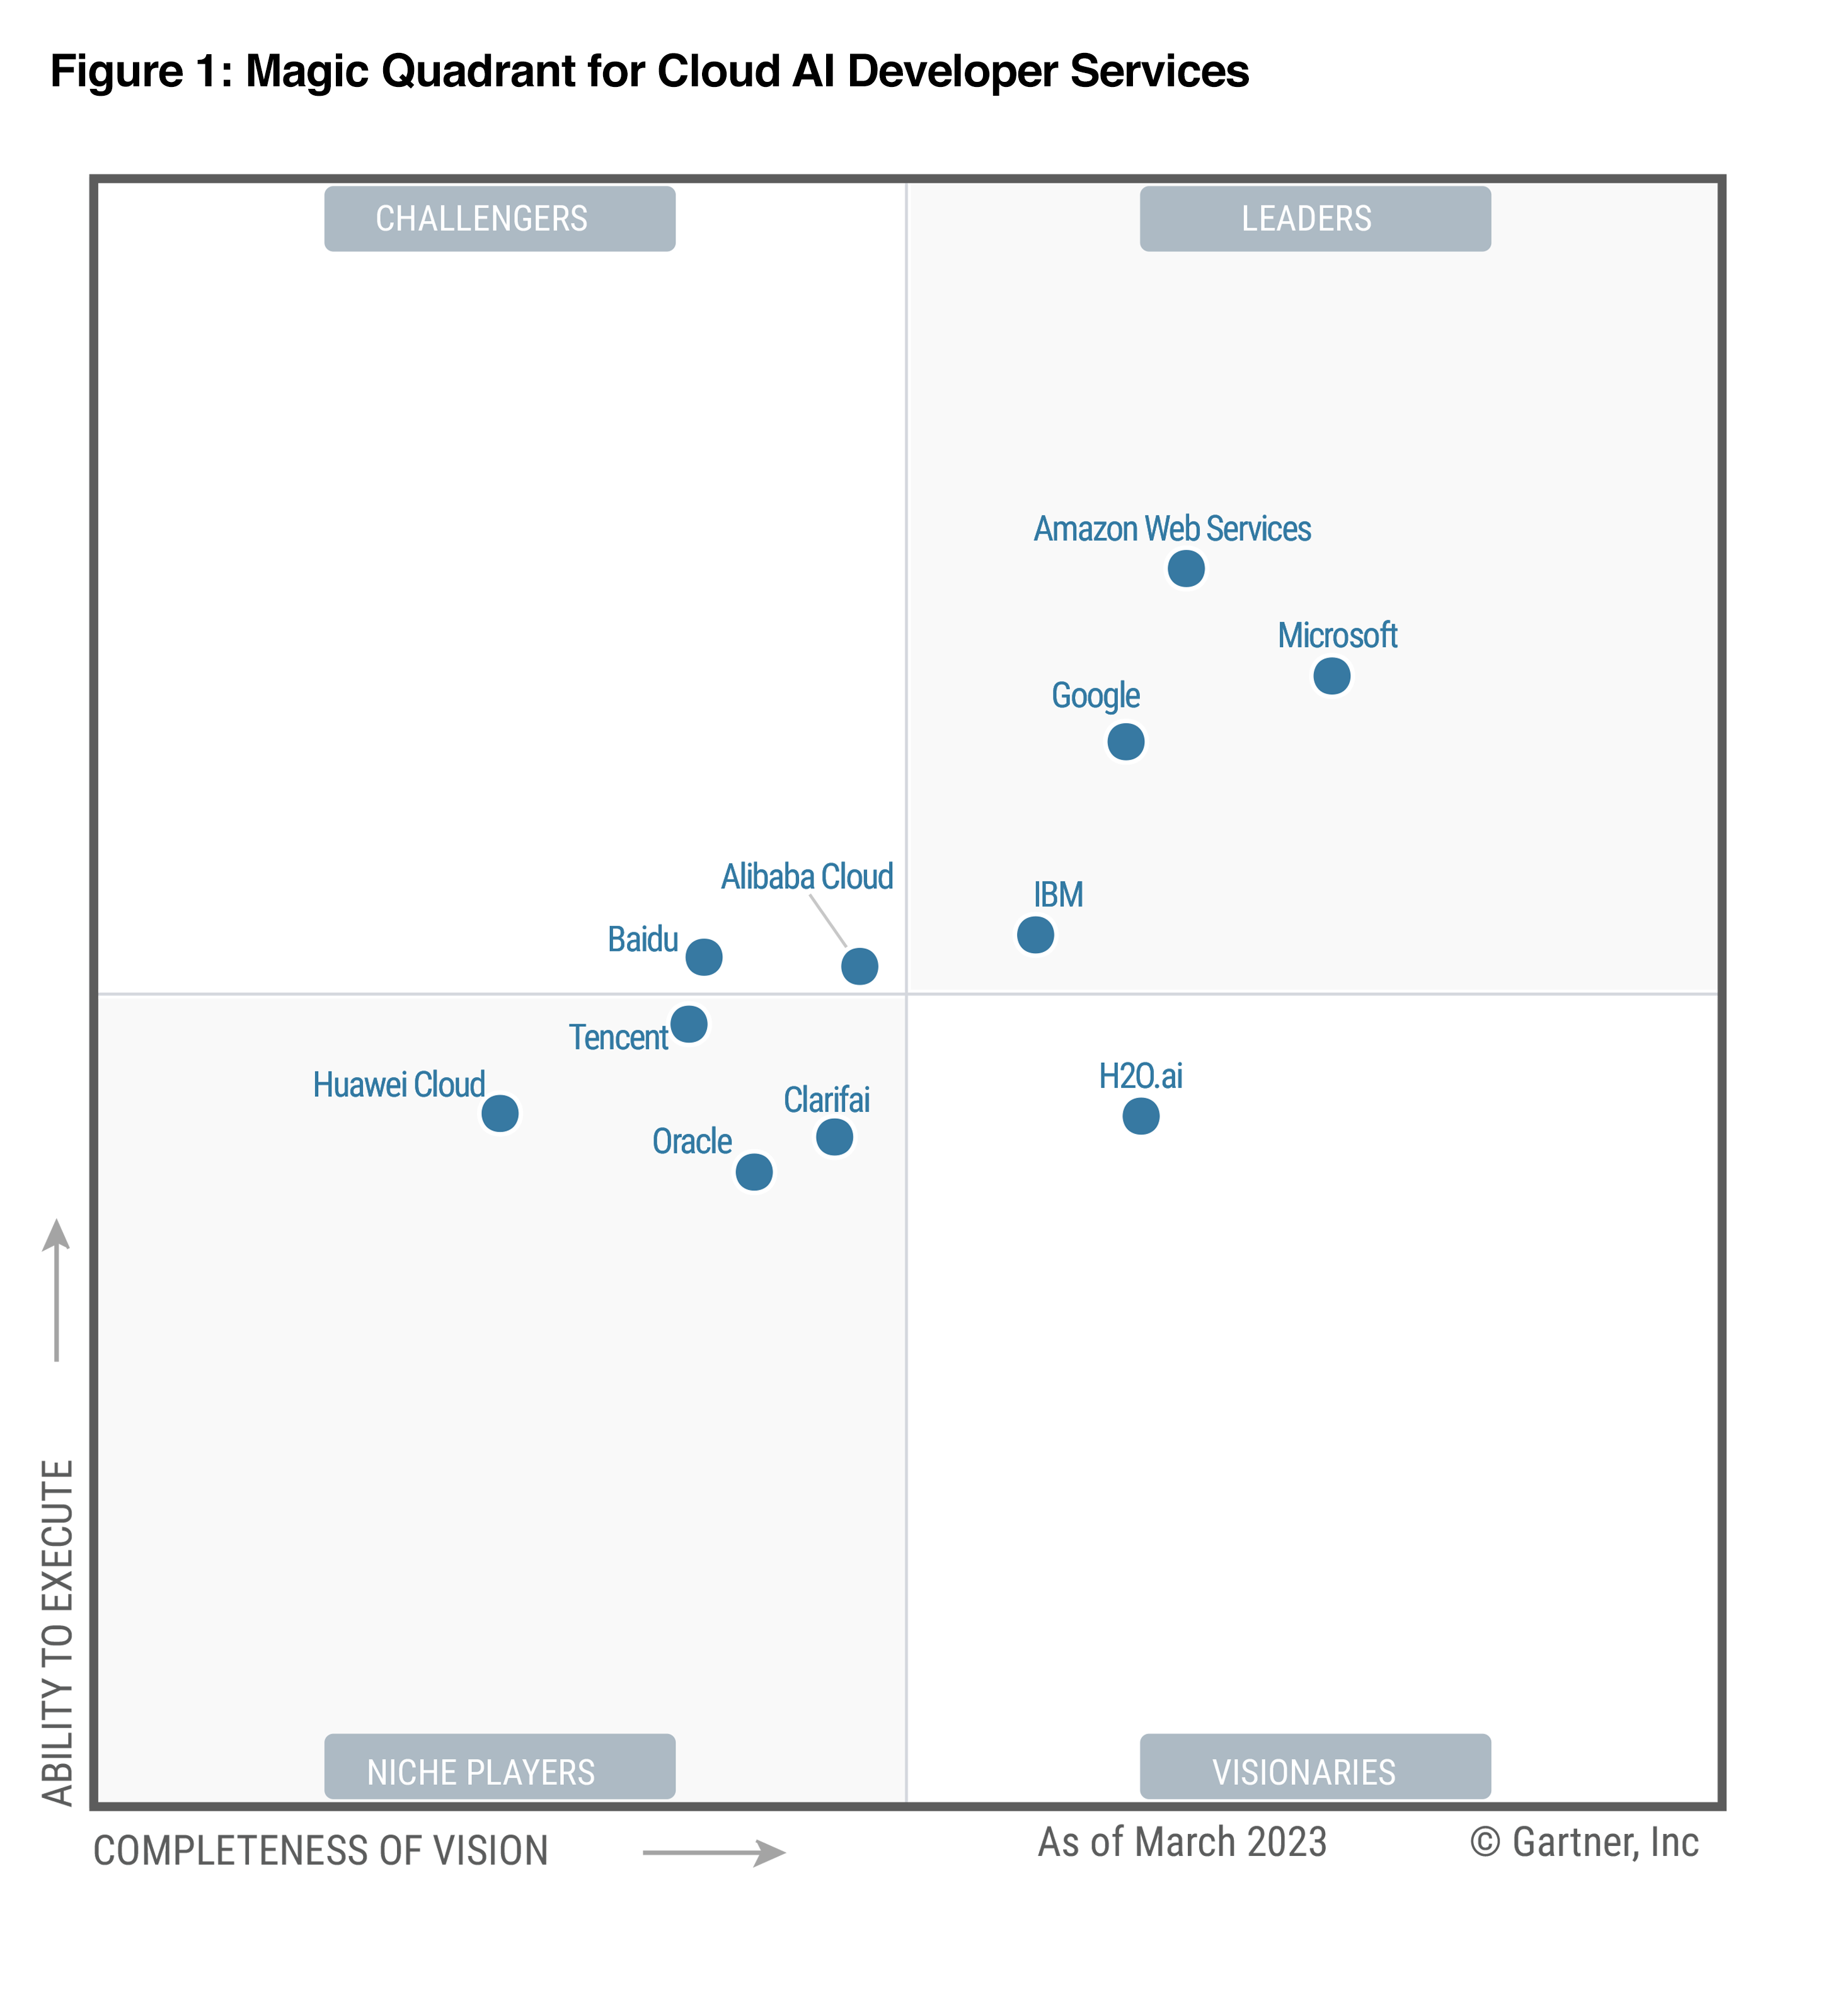
\includegraphics[width=0.6\textwidth]{images/AWSMagicQuadrantForCloud.png}  % Sostituisci 'nome_immagine' con il nome del tuo file immagine e l'estensione
  \caption{The Gartner Magic Quadrant for Cloud Infrastructure and Platform Services \cite{GartnerMagicQuadrant}}
  \label{fig:AWSMagicQuadrantForCloud}
\end{figure}

The infrastructure exhibits several key attributes contributing to its robustness and efficiency: 
\begin{itemize} 
  \item \textbf{Security:} The infrastructure undergoes 24/7 monitoring to ensure the confidentiality, integrity, and availability of data. All data flowing across the AWS global network is automatically encrypted at the physical layer before leaving secured facilities.
  \item \textbf{Availability:} To ensure high availability and isolate potential issues, applications can be partitioned across multiple AZs (Availability Zones) within the same region, creating fully isolated infrastructure partitions.
  \item \textbf{Performance:} AWS Regions offer low latency, low packet loss, and high overall network quality. This is achieved through a fully redundant 100 GbE fiber network backbone, often providing terabits of capacity between Regions.
  \item \textbf{Scalability:} The AWS Global Infrastructure allows companies to take advantage of the virtually infinite scalability of the cloud. This enables customers to provision resources based on actual needs, with the ability to instantly scale up or down according to business requirements.
  \item \textbf{Flexibility:} The AWS Global Infrastructure provides flexibility in choosing where and how workloads are run, whether globally, with single-digit millisecond latencies, or on-premises.
  \item \textbf{Global Footprint:} AWS boasts the largest global infrastructure footprint, continually expanding at a significant rate.
\end{itemize}
Thanks to its expertise and qualifications, Storm Reply is able to provide the above features to its customers, offering a comprehensive consultancy service for managing cloud infrastructures.

\section{Thesis Objective}
In the automotive context, the use of Software Defined Vehicle (SDV) plays a crucial role in terms of cost, innovation and safety. The objectives of the thesis are intertwined with the opportunities offered by Software Defined Vehicle technology, for instance addressing the primary challenge of overcoming the current difficulties associated with the presence of different specialized hardware platforms on the same vehicle, to make the vehicle a more efficient and safer device based on software as a fundamental element.

One of the main objectives of this thesis is to propose the opportunity offered by Software Defined Vehicle solution capable of eliminating various phases of the software production pipeline. This would result in significant time and cost savings, enabling the investment of these resources in other areas.

From a practical standpoint, the project's goal is to provide, through the use of AWS services, a cloud infrastructure capable of managing the Software Defined Vehicle both in terms of software production and data analysis.

The work begins with an overview of the state of the art of software development in the automotive world, comparing the goals of the future with the techniques used in the past. For this purpose, the weaknesses of the sector are explained in order to highlight the advantages of SDV technology.Next, some definitions of the technologies that can bring the development of a paradigm shift in SDV benefits are provided. Finally, an example of an initiative proposed as a first attempt to standardize the SDV concept is presented, namely the SOAFEE project.

The work continues with an introduction to cloud computing, which is the programming approach that accompanied the entire project from beginning to end. The characteristics of this technique are analyzed, especially the advantages it can bring, and the example of how AWS manages to best enhance the potential of cloud computing is shown. Special attention is given to the security aspect, as it is a fundamental objective of the thesis topic, but also central element of the idea behind the cloud development of the AWS company and the project partner company.

Moving towards the description of the implementation of the practical project, it is possible to arrive at the exploration of the AWS services used. In order to make the realization of the project possible, as described several times throughout the thesis, it is necessary to rely on this type of service. With the aim of introducing the characteristics of the services used, an extensive descriptive list is provided.

The last part of the thesis deals with the actual implementation of the project, with the purpose of providing a concrete and working example of what has been described in the previous chapters. The implementation begins with the creation from scratch of a device capable of simulating telematic data, develops in the construction of a cloud infrastructure with the services mentioned above, and ends with the exploration of the tool used for data analysis.

Finally, to conclude the research, the results of the final presentation of the operation of the whole system on a real device are shown. In addition, a final evaluation of the whole project is made and the future possibilities opened by the work are shown.